\section{Materials and Methods}\label{sec:materials-and-methods}

\subsection{Motivating Datasets}\label{sec:motivating-datasets}
A data object is a collection of information. Types of data objects include collections of images, documents, spatiotemporal recordings, or genomics information. 
Data objects are often sampled and structured into a table or matrix for analysis, modeling and inference. 
We present three data objects that motivate our method of computing a proper latent feature representation:

{\color{purple}Need to be more clear that we are working with functonal data.}

\subsubsection{Glaucoma Data}




\subsubsection{Proteomic Gels Data}


\subsubsection{MNIST Digits Data}

\begin{figure}
    \centering
    \includegraphics[width=1\textwidth]{example-image-c}
    \caption{
    A sample observation from each of our three motivating datasets.
    \textbf{(a)}: A sample glaucoma image, representing a polar azimuthal projection of MPS functionsfor a single eye at one IOP level.
    \textbf{(b)}: A sample 2D gel electrophoresis image, showing proteomic content in the brain tissue of a rat.
    \textbf{(c)}: A sample MNIST digit image, which is a $28 \times 28$ pixel greyscale image of single handwritten digit.}
    \label{fig:enter-label}
\end{figure}

\subsection{Latent Feature Representations}

\add{Suppose that we have $N$ observations of object data, denoted by $X_1 (t), \dots, X_N(t)$, where $t$ indexes a location on a continuous domain $\mathcal{T}$ over which the objects are defined.
For time-varying curves, $\mathcal{T}$ is generally a closed subset of the real line that represents a (normalized) time interval.
However, as exemplified in our three motivating datasets, the domain $\mathcal{T}$ can be multi-dimensional to represent locations in an image or surface, and it can also be non-Euclidean ({see Glaucoma data/ \textcite{lee_bayesian_2019}}).
We assume that each observation is measured on a common\footnote{In practice, the measurement grids of individual observations need not be identical if they are all sufficiently fine such that interpolation onto a common, fine grid is feasible.}, ordered grid of $T$ points in $\mathcal{T}$, denoted by $\mathbf{t} = \left(t_1, \dots, t_T\right)^\top$, and we let $X_i(\mathbf{t}) = \left(X_i(t_1), \dots, X_i(t_T)\right)^\top$.
Then, we can represent the observed data in the $N \times T$ data matrix $\mathbf{X}$, which contains the vectors $X_1(\mathbf{t}), \dots, X_N(\mathbf{t})$ in its rows.
We refer to the $T$-dimensional space of features in which the observed data are represented as the \emph{data space}.}

\add{We define a \emph{latent feature representation} as a method that transforms each observation from the data space\footnote{If we have have representation of the underlying object $X_i(t)$ that does not involve measurement on a grid, the transformation can be defined on the object itself as $f_{K} \left(X_i(t)\right) = \left(X_{i1}^*, \dots,  X_{iK}^* \right)^\top$.} to a new space of latent features, called the \emph{representation space}.
Mathematically, we define the latent feature representation of the $i$th observation as
$$
f_{K} \left(X_i(\mathbf{t})\right) = \left(X_{i1}^*, \dots,  X_{iK}^* \right)^\top,
$$
where the number of features $K$ defines the dimensionality of the representation space and can range between $1$ and some possible maximum $K_{max}$.
When $K \ll T$, we say that the latent feature representation is \emph{sparse}.
As we expand on in Section {\color{purple}X}, the dimension of the representation space is generally selected according to some criteria of information loss.
We also require that there exists an inverse transformation $f^{-1}_K$ that maps each observation from the representation space back to the data space as
$$
\widehat{X}_i(\mathbf{t}) = f_{K}^{-1} \left( \left(X_{i1}^*, \dots,  X_{iK}^* \right)^\top \right).
$$}

\add{Linear transformations of the form $f_{K} \left(X_i(\mathbf{t})\right) = \mathbf{A} X_i(\mathbf{t})$, for some $K \times T$ transformation matrix $\mathbf{A}$, are often used in practice.
For example, it is common to represent a functional observation $X_i(t)$ as a linear combination of a set of basis functions $\{\phi_k(t)\}_{k=1}^K$, which defines the inverse transformation
$$
\widehat{X}_i(\mathbf{t}) = \sum_{k=1}^K X_{ik}^* \phi_k(\mathbf{t}) = \boldsymbol{\Phi} \left(X_{i1}^*, \dots,  X_{iK}^* \right)^\top,
$$
where $\boldsymbol{\Phi} = \left[\phi_1(\mathbf{t}) | \dots | \phi_K(\mathbf{t}) \right]$ and the latent features $X_{ik}^*$ are basis coefficients. 
When these basis coefficients are computed by ordinary least squares, the linear transformation matrix defining the latent feature representation $f_K$ is of the form $\mathbf{A} = \left( \boldsymbol{\Phi}^\top \boldsymbol{\Phi} \right)^{-1} \boldsymbol{\Phi}^\top$.
When the matrix of basis function evaluations $\boldsymbol{\Phi}$ is orthogonal, $\mathbf{A} = \boldsymbol{\Phi}^\top$, i.e., the transformation $f_K$ is simply right multiplication by this matrix.
However, in general, there is no need for the transformation $f_K$ to be orthogonal or even linear, and non-linear transformations may be preferred for certain types of data.}


\subsection{Assessing Losslessness via Generalization Error}

\add{Although modelling is performed in the representation space due to its attractive properties, we often want to transform modelling results back to the data space for inference, interpretation and visualisation. 
As such, the accuracy and interpretation of an analysis depends on the degree of information that is preserved when moving between the data and representation spaces for a given latent feature representation.
In what follows, we characterise the degree of information loss of a latent feature representation on a full dataset.
}



\subsection{Characterising Information Loss}
We characterise the degree of information loss of a latent feature representation for each individual observation as
$$
\text{Loss} \left( f_K(X_i(t)) \right) = \lVert  X_i(\mathbf{t}) - f^{-1}_{K}(X_{ik}^*) \rVert,
$$
where $\lVert \boldsymbol{\cdot} \rVert$ denotes a measure (e.g., $\mathcal{L}_2$ norm) such that $\lVert  X_i(\mathbf{t}) - f^{-1}_{K}(X_{ik}^*) \rVert$ defines a distance between $X_i(\mathbf{t})$ and $f^{-1}_{K}(X_{ik}^*)$ \parencite{morris_comparison_2017}.
We say that the transformation $f_K$ is \emph{lossless} for the $i$th observation $X_i(t)$ if
$$
\text{Loss} \left( f_K(X_i(\mathbf{t})) \right) = 0,
$$
and lossless for the full dataset $X_1(t), \dots, X_N (t)$ if
$$
\text{Loss} \left( f_K(X_i(\mathbf{t})) \right) = 0 \quad \forall \quad  i = 1, \dots, N.
$$
That is, we only refer to a latent feature representation as lossless for a given dataset if the representation is near lossless for every individual observation in that dataset.
More generally, we can allow some tolerance of information loss and say that
the transformation $f_K$ is \emph{near-lossless} for the $i$th observation $X_i(t)$ if
$$
\text{Loss} \left( f_K(X_i(\mathbf{t})) \right) < \epsilon,
$$
for a chosen tolerance level $\epsilon$. 
Similarly, we say that the transformation $f_K$ is near-lossless for the full dataset only if each individual observation achieves this tolerance level, that is
$$
\text{Loss} \left( f_K(X_i(\mathbf{t})) \right) < \epsilon \quad \forall \quad  i = 1, \dots, N.
$$
In this case, it is important to note that the distinction between this definition and a measure such as the average of individual losses $\frac{1}{N}\sum_{i=1}^N \text{Loss} \left( f_K(X_i(\mathbf{t})) \right)$.
For example, Figure \ref{fig:ind-losses} displays the distribution of individual information losses on a dataset sample dataset of a PCA latent of varying dimensions.
In this case, we are using the squared correlation measure as our loss, so a value $0$ means the representation captures no information and a value of $1$ means that the representation is lossless.
The grey points represent the individual observations' losses, whereas the red squares indicate the average loss.
The figure highlights the information that can be hidden when on a single measure is used to describe the full distribution of losses. For example, at $k = 1$ the average loss is at $0.4$ but there are observations with individual losses at almost $0$.


\begin{figure}
    \centering
    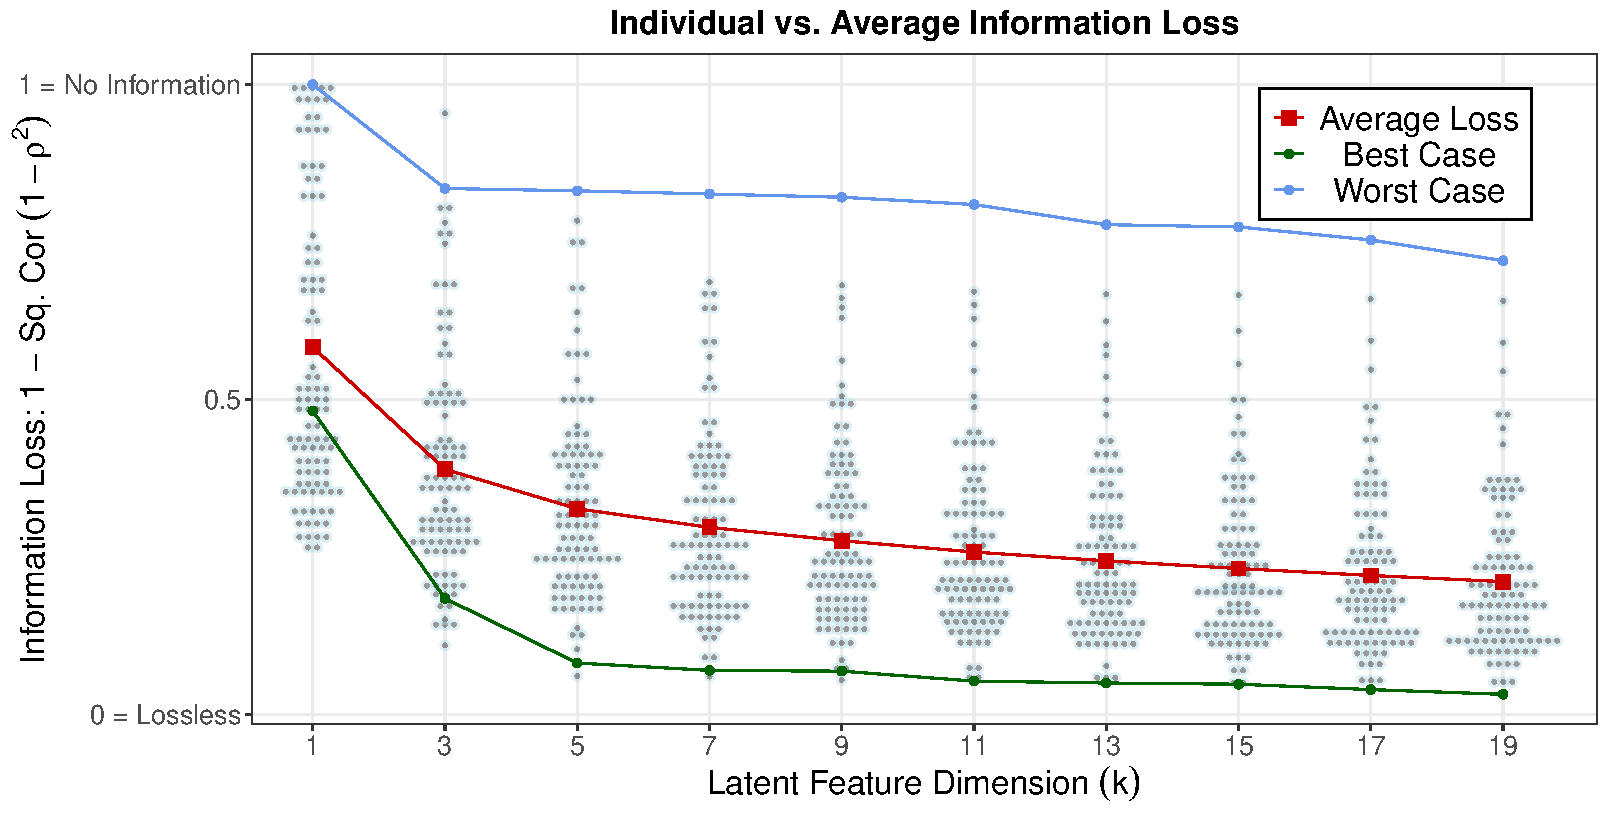
\includegraphics[width=0.75\textwidth]{figures/info-loss.pdf}
    \caption{Phoneme data \textcite{hastie_elements_2009}. \add{\textbf{To Do: Trace minimum, maximum and quantiles.}}}
    \label{fig:ind-losses}
\end{figure}
\newline

It often suffices to achieve this tolerance level for the majority of observations, i.e., there may be a small number of observations for which achieving near-losslessness is not possible. We can extend our definition to accommodate this notion by introducing a \emph{qualifying criterion (qc)}, which is the proportion of observations in the dataset that achieve near-losslessness at a given tolerance level.
Mathematically, we can define the transformation $f_K$ as near-lossless at a tolerance level $\epsilon$ and a qualifying criterion $qc$\footnote{Could try to write as $\frac{\sum_{i \text{ s.t. } \text{Loss} \left( f_K(X_i(\mathbf{t})) \right) < \epsilon }1}{N}$?}
$$
\frac{| \{x \in \{X_i(\mathbf{t})\}_{i}^N : \text{Loss} \left( f_K(x) \right) < \epsilon \} |} 
{N}
\geq qc,
$$
where the notation $|S|$ represents the cardinality (i.e., number of elements) in a set $S$.}
\subsubsection{Generalization Error of Individual Data Objects}
\subsubsection{Performance Across Quantiles of Individual Data Objects}